\pagenumbering{gobble}  % Pas de numérotation
\begin{titlepage}
    \vspace*{-10px}
    
\includegraphics[height=80px]{Images/logo_phelma.pdf}
    \vspace*{-80px}
\begin{flushright}
    \vspace*{-10px}
    
\includegraphics[height=80px]{Images/Logo_Neel.pdf}
\end{flushright}

\vspace*{1.5cm}
\begin{center}
\LARGE{\textsc{Félix Piédallu}}\\[1.5cm]

\rule{\linewidth}{0.5mm}\\[0.4cm]
{\huge{\bfseries Rapport de Projet de Fin d'Études}\\[0.4cm]
Caractérisation de pointes fibrées pour nano-pinces optiques et plasmoniques\\[0.4cm]}
\rule{\linewidth}{0.5mm}\\[0.5cm]

\large{\textsc{Filière PNS 2015-2016}}\\[2cm]

\Large{Au sein de l'équipe Nano-Optique et Forces}\\[1cm]

\Large{Sous la direction de Jochen \textsc{Fick}}\\[1cm]

\large{Du 22 Février 2016 au 22 Juillet 2016}\\[2cm]

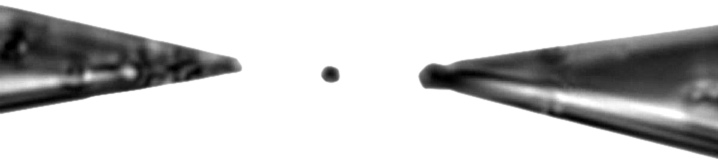
\includegraphics[width=\textwidth]{Images/Illustration.png}\\[1cm]


\end{center}
\end{titlepage}
\newpage\null\thispagestyle{empty}\newpage
% Remerciements
\vspace*{\stretch{1}}
\begin{center}
\textsc{\Large Remerciements}
\end{center}

\vspace{0.5cm}
Je tiens tout d'abord à remercier mon maître de stage, Jochen \textsc{Fick}, qui m'a donné l'opportunité d'effectuer mon projet de fin d'études au sein de l'équipe Nano-Optique et Forces à l'Institut Néel. Je remercie également Grenoble INP Phelma pour m'avoir permis d'obtenir, à travers mes études et ce stage, une formation scientifique de qualité.
Enfin, je remercie l'ensemble des personnes avec qui j'ai pu, d'un point de vue professionnel et personnel, échanger lors de ce stage: Jean-François \textsc{Motte} et Gwénaëlle \textsc{Julie}, avec qui j'ai pu travailler en salle blanche pour la réalisation des pointes métallisées, ainsi que les membres des équipes NOF et QNES que j'ai eu la chance de côtoyer: Aurélien \textsc{Drezet}, Guillaume \textsc{Bachelier}, Herman \textsc{Sellier}, Martin \textsc{Berthel}, Nicolas \textsc{Chauvet}, Guillaume \textsc{Laurent}, Maëliss \textsc{Ethis-De-Corny}, Aline \textsc{Pham}, Vincent \textsc{Morice} et Vincent \textsc{Delmas}.

\vspace*{\stretch{3}}

\tableofcontents        % Table des matières avec liens, générée automatiquement.
\newpage
\listoffigures
\pagenumbering{arabic}  % Numérotation de retour !
